
%%%%%%%%%%%%%%%%%%%%%%%%%%%%%%%%%%%%%%%%%%%%%%%%%%%%%%%%%%%%%%%%%%%%%%%%%%%%%
%%%%% Traversing a mesh %%%%%%%%%%%%%%%%%%%%%%%%%%%%%%%%%%%%%%%%%%%%%%%%%%%%%
%%%%%%%%%%%%%%%%%%%%%%%%%%%%%%%%%%%%%%%%%%%%%%%%%%%%%%%%%%%%%%%%%%%%%%%%%%%%%
\begin{frame}
\pointedsl{
	Exploration
}
\end{frame}

% TODO
% Content:
% 1. Iterators (vertex, edges, half-edges, faces)
% 2. Manual: looping over the boundary
% 3. Manual: looping over edges/vertices of a face
% 4. Manual: 1-ring vertex traversal
% 5. Circulators (vertex, edges, half-edges, faces)

%%%%%%%%%%%%%%%%%%%%%%%%%%%%%%%%%%%%%%%%%%%%%%%%%%%%%%%%%%%%%%%%%%%%%%%%%%%%%
\begin{frame}[fragile]
\frametitle{Iterators}
\misc{
	\textbf{Iterators} are used to traverse all the elements of a specific type (\emph{vertices}, \emph{halfedges}, \emph{edges} or \emph{faces}).
}
\begin{lstlisting}
// iterating over all vertices
Surface_mesh::Vertex_iterator vit, vend;
for(vit = mesh.vertices_begin(),
    vend = mesh.vertices_end();
    vit != vend; ++vit){
  Vertex v = *vit;
  // do something with vertex v
}
\end{lstlisting}
\end{frame}

\begin{frame}[fragile]
\frametitle{Iterators and ordering}
\begin{lstlisting}
// iterating over all half-edges
Surface_mesh::Halfedge_iterator hit;
hit = mesh.halfedges_begin();

// iterating over all edges
Surface_mesh::Edge_iterator eit;
eit = mesh.edges_begin();

// iterating over all faces
Surface_mesh::Face_iterator fit;
fit = mesh.faces_begin();
\end{lstlisting}
\misc{
	Iterators traverse elements in the order they are stored in memory.
	\textbf{You should not expect any ordering.}
}
\end{frame}

\begin{frame}
\frametitle{Iterators}
\begin{center}
	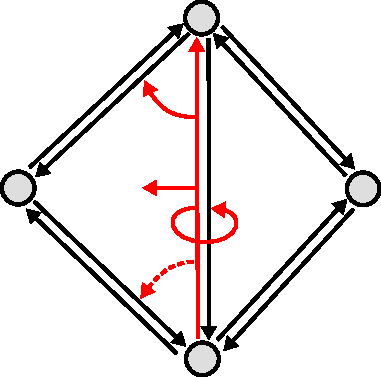
\includegraphics[width=0.5\textwidth]{figures/halfedge-connectivity}
\end{center}
\misc{
	Meshes are made of \emph{vertices}, \emph{edges} and \emph{faces}.
	
	Here, each edge is made of two half-edges (directed edges).
}
\end{frame}

\begin{frame}
\frametitle{Half-edges connectivity}
\begin{columns}[c]
  \begin{column}{0.4\textwidth}
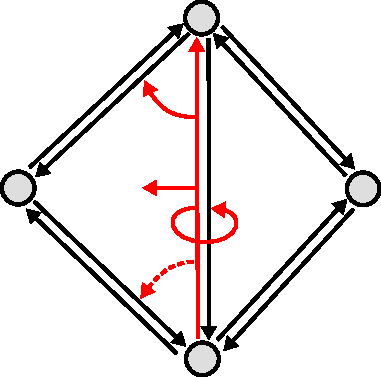
\includegraphics[width=\textwidth]{figures/halfedge-connectivity}
  \end{column}
  \begin{column}{0.6\textwidth}
\begin{itemize}
	\color{black}
	\item[\color{black}\textbullet] Each \textbf{vertex} is linked to an outgoing half-edge
	\item[\color{black}\textbullet] Each \textbf{face} is linked to an incident half-edge
	\item[\color{black}\textbullet] Each \textbf{half-edge} has \begin{itemize}
		\color{black}
		\item[\color{black}\textbullet] A next and previous half-edge
		\item[\color{black}\textbullet] A target vertex it points to
		\item[\color{black}\textbullet] An incident face
		\item[\color{black}\textbullet] An opposite half-edge\\(on the same edge)
	\end{itemize}
\end{itemize}
  \end{column}
\end{columns}
\end{frame}

\begin{frame}[fragile]
\frametitle{Half-edges code}
\begin{columns}[c]
  \begin{column}{0.4\textwidth}
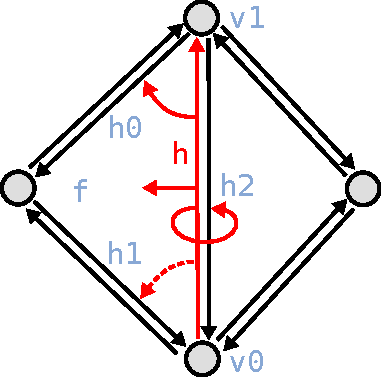
\includegraphics[width=\textwidth]{figures/halfedge-queries}
  \end{column}
  \begin{column}{0.6\textwidth}
  \lstset{ 
  	numbers=none, 
  	xleftmargin=0cm, 
  	xrightmargin=0cm
  }
\begin{lstlisting}
using Surface_mesh::Halfedge;
using Surface_mesh::Face;
using Surface_mesh::Vertex;

// the starting half-edge
Halfedge h;
// the connected elements
Halfedge h0, h1, h2;
Face f;
Vertex v0, v1;
\end{lstlisting}
  \end{column}
\end{columns}
\end{frame}

\begin{frame}[fragile]
\frametitle{Half-edges code}
\begin{lstlisting}
// next half-edge
h0 = mesh.next_halfedge_handle(h);
// previous half-edge
h1 = mesh.prev_halfedge_handle(h);
// opposite half-edge
h2 = mesh.opposite_halfedge_handle(h);
// incident face
f = mesh.face_handle(h);
// vertex at source
v0 = mesh.from_vertex_handle(h);
// vertex pointed by h
v1 = mesh.to_vertex_handle(h);
\end{lstlisting}
\end{frame}
